\documentclass[a4paper,10pt,twocolumn]{article}
\usepackage[utf8]{inputenc}
\usepackage{graphicx}
\usepackage[center]{caption}
\usepackage{subcaption}

% \usepackage[top=3cm, bottom=3cm, left=2cm, right=2cm]{geometry}

%---------------------------------------------
% Font packages
%---------------------------------------------
% \usepackage{lmodern}
% \usepackage{concmath}
% \usepackage{cmbright}
% \usepackage{kpfonts}
% \usepackage[adobe-utopia]{mathdesign}
\usepackage{fouriernc}
\usepackage[T1]{fontenc}

%---------------------------------------------
% Math environment packages & command
%---------------------------------------------
\usepackage{amsmath}
\usepackage{amssymb}
\usepackage{array}
\usepackage{mathrsfs}
\usepackage{array}
\def\sgn{\mathop{\rm sgn}\nolimits} 


%---------------------------------------------
% item option
%---------------------------------------------
\renewcommand{\labelitemi}{-}


%---------------------------------------------
%HEADER & FOOTER
%---------------------------------------------
\usepackage{fancyhdr}
\pagestyle{fancy}

\renewcommand{\headrulewidth}{.15pt}
\fancyhead[C]{{Homework Assignment 2}} 
\fancyhead[L]{Page \thepage \ of \pageref{LastPage}}
\fancyhead[R]{MF2007}

\renewcommand{\footrulewidth}{.15pt}
\fancyfoot[C]{\thepage} 
% \fancyfoot[L]{truc}
% \fancyfoot[R]{\leftmark}

\usepackage{lastpage}

%---------------------------------------------
% two column option
%---------------------------------------------
\setlength{\columnsep}{1cm}

%---------------------------------------------
% Table of content
%---------------------------------------------
\usepackage[colorlinks,linkcolor=black, citecolor=black]{hyperref}

%opening
\title{MF2007: Dynamic \& Motion Control \\ Homework 1}
\author{Kilian \textsc{Demeulemeester}, Jeremy \textsc{Pouech} \\ \texttt{\{kiliande,pouech\}@kth.se}}

\begin{document}

\setlength\parindent{0em}

\maketitle

\tableofcontents

\begin{abstract}
 This paper summarizes our work on servo control, code implementation on a microprocessor and analysis of the robustness to parameters uncertainties and sensor noise. The first and second parts use the result from workshop A about how to control a DC-motor in position, improving the controller by using a model following block and a trajectory planner. The last part deals with closed loop poles positionning in the case of a valved controlled hydraulic cylinder.
\end{abstract}
  

\part*{Servo Control} 
\addcontentsline{toc}{part}{Servo Control}

\section*{Model following control}
\addcontentsline{toc}{section}{Model following control}

\subsection*{Level 1}
\addcontentsline{toc}{subsection}{Level 1}

Here, we will design a model following controller by inverting the process model in the time domain.

The control structure and the model following block are depicted in Figure \ref{contStruct}.
z
\begin{figure}[t!p]
\begin{center}
  \begin{subfigure}[b]{\columnwidth}
  \includegraphics[trim=125 40 150 40,clip=true,height=\linewidth,angle=270]{fig/modelFollowing.eps}
 \caption{Model following for the DC-motor}
  \end{subfigure}
    \begin{subfigure}[b]{\columnwidth}
  \includegraphics[trim=125 0 150 25,clip=true,height=\linewidth,angle=270]{fig/modelMotorServo1.eps}
   \caption{Control structure for the DC-motor}
  \end{subfigure}
  \caption{Model following and control structure for a DC-motor}
 \label{contStruct}
\end{center}
\end{figure}

Since the DC-motor model we used is a second order system, the reference position must be two times differentiable. 

The trajectory planner is design using the fastest possible positionning:
\begin{equation}a_{max} = \frac{\pm M_{max}}{J}\end{equation}
\begin{equation}v_{max} = \pm \frac{U_{max} - \frac{R}{k_\varphi} F_c}{\frac{R d}{k_\varphi} + k_\varphi}\end{equation}

With:

$M_{max}$ : maximum torque of the motor

$v_{max}$ : maximum reachable velocity of the DC-motor, computed with the DC motor model equations.

The reference signal is computed using the following equations:

  Let $t_1 = \frac{v_{max}}{a_{max}}, t_2 = \frac{Rs}{v_{max}}  \text{ and } t_1' = \sqrt{\frac{Rs}{a_{max}}}$\\
  \begin{equation}
  a(t) = \left\{ \begin{array}{lcl} a_{max} & , & t < t_1 \\
				      0 & , & t_1 < t < t_2 \\ 
				  -a_{max} &,& t_2 < t < t_1 + t_2 \\
				  0 & , & t>t_1 + t_2
		  \end{array} \right.\text{ , if } t_1 < t_2
  \end{equation}
  \begin{equation}
  a(t) = \left\{ \begin{array}{lcl} a_{max} & , & t < t_1' \\
				  -a_{max} &,& t_1' < t < 2t_1'\\
				  0 & , & t>2t_1'
		  \end{array} \right.\text{ , if } t_1 > t_2
  \end{equation}


The reference signal is then created as depicted in Figure \ref{trajplan}.

\begin{figure}[t!p]
  \begin{center}

  \begin{subfigure}[b]{\columnwidth}
  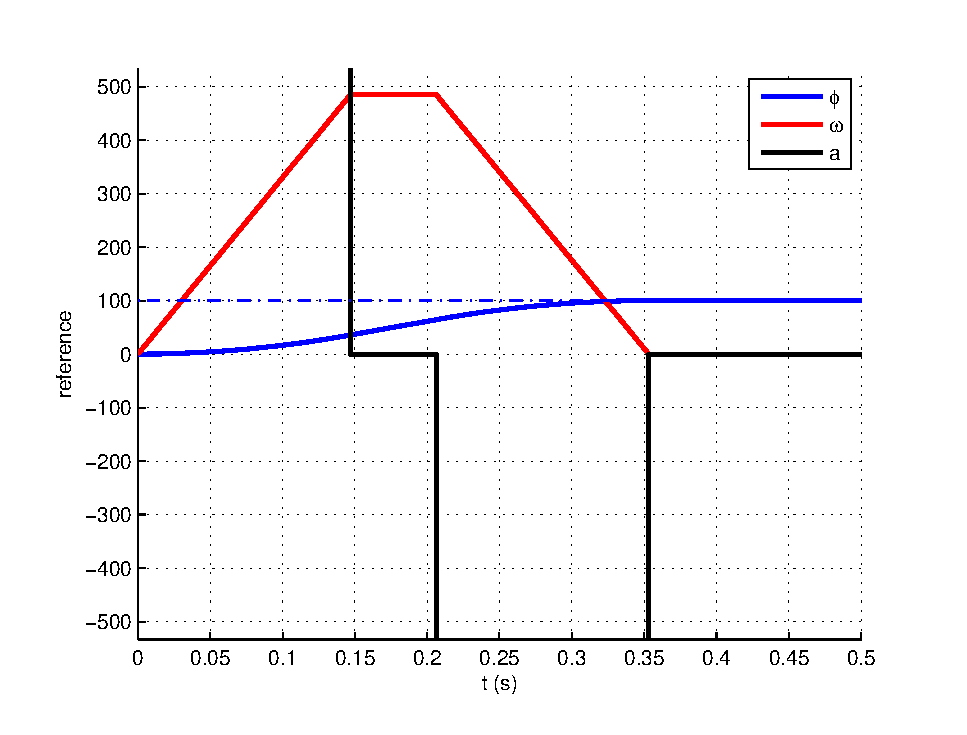
\includegraphics[width = \columnwidth]{fig/trajPlanref100.eps}
  \caption{Reference signal for $Rs = 100$ [rad]}
  \end{subfigure}
  \vspace{\fill}
  \begin{subfigure}[b]{\columnwidth}
  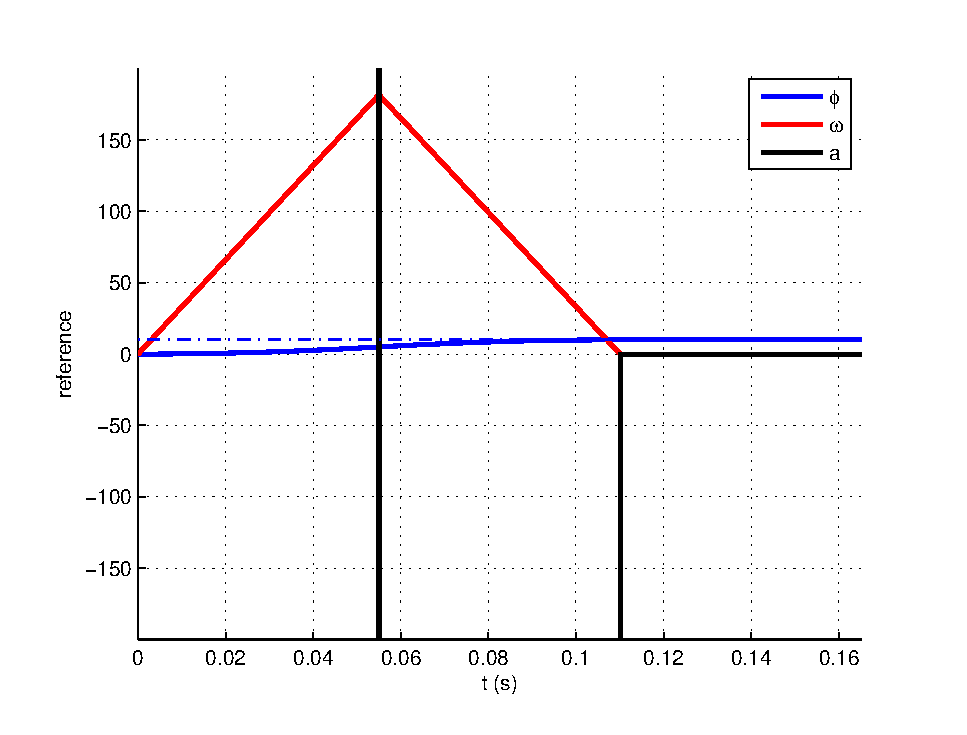
\includegraphics[width = \columnwidth]{fig/trajPlanref10.eps}
  \caption{Reference signal for $Rs = 10$ [rad]}
  \end{subfigure}
\caption{Reference signal}
\label{trajplan}
\end{center}
\end{figure}


Once the reference signal is designed, we simulate the system (simulation and real-case). Figure \ref{resultModelfollowing} shows the results.
 
The Servo control model leads to an excellent control law of the motor for the two set points. Since the trajectory computed by the trajectory planner is completly reachable by the real-motor (no saturation), the planned trajectory and the real one are almost completly merged.

\textbf{Remark:} In order to be sure of our control design, we reduced the value of $a_{max}$ and $v_{max}$ to $75\%$ of the value computed theoretically. Indeed, using the maximum value of those value drive the motor to a dangerous area.

\begin{figure}[ht]
  \centering
  \begin{subfigure}[b]{\linewidth}
   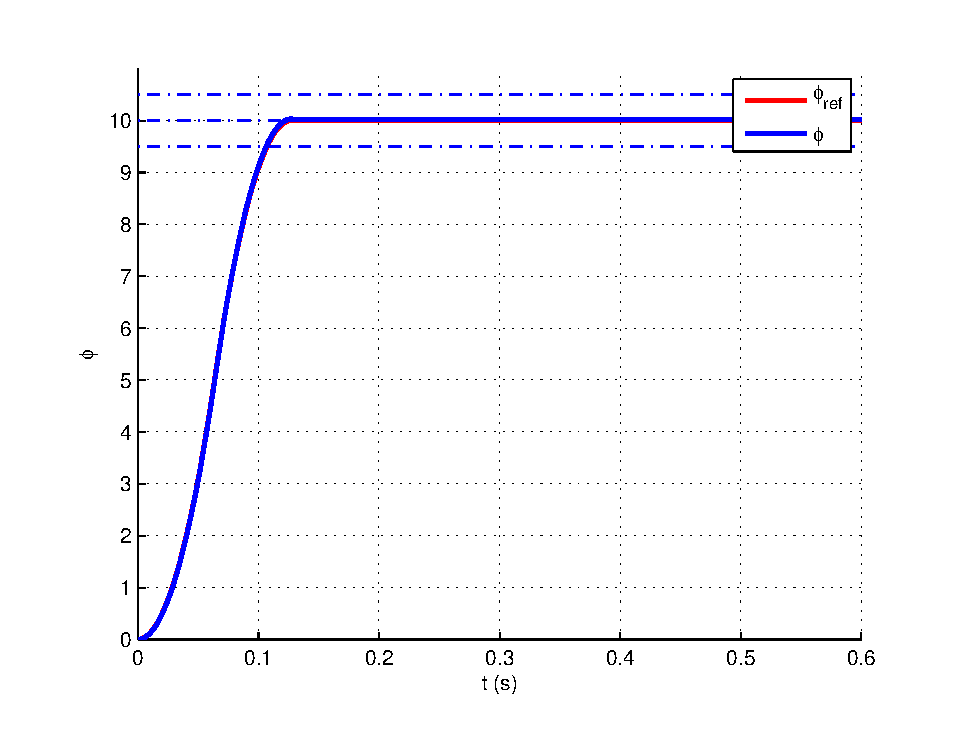
\includegraphics[width=\columnwidth]{fig/resultModelControl10.eps}
   \caption{$Rs = 10$[rad]}
  \end{subfigure}
  \begin{subfigure}[b]{\linewidth}
  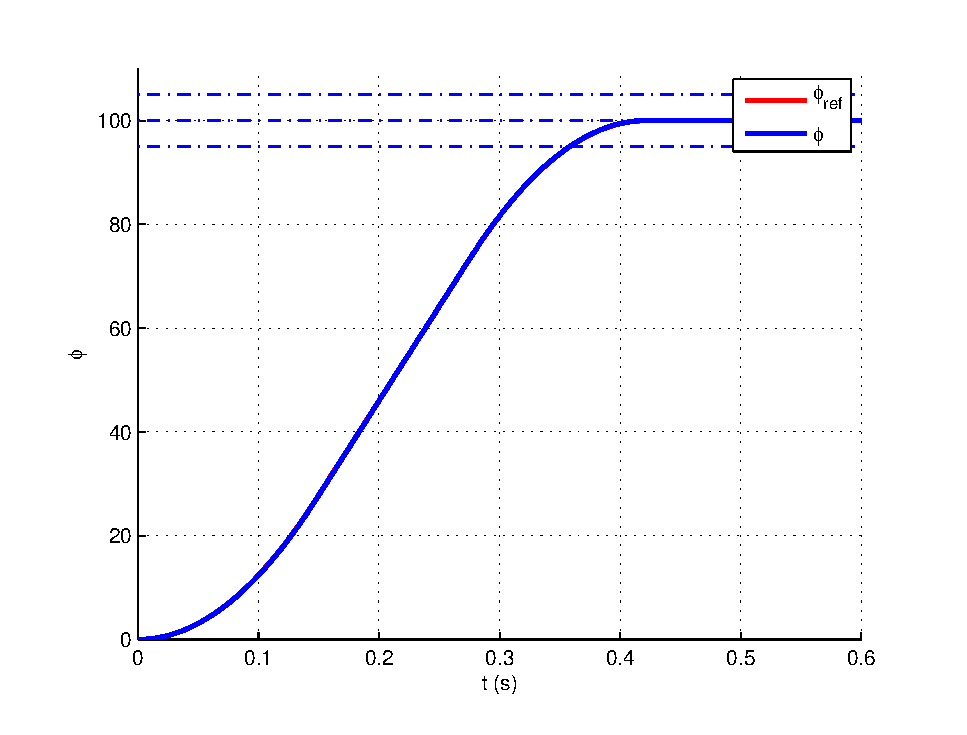
\includegraphics[width=\columnwidth]{fig/resultModelControl100.eps}
   \caption{$Rs = 100$[rad]}
  \end{subfigure}

 \caption{Position controller}
 \label{resultModelfollowing}
\end{figure}



	

\part*{Writing controller code} 
\addcontentsline{toc}{part}{Writing controller code}

%------------------------------------------------
% 		LEVEL 1
%------------------------------------------------
\subsection*{Level 1}
\addcontentsline{toc}{subsection}{Level 1}

The embedded Matlab implementation leads to the exact same result than the implementation using ordinary Simulink blocks. Indeed, since we use a discretize controller, transposing the simulink code to the embedded Matlab implementation produce the a code with the same behavior as the one produced by Simulink.

Figure \ref{embedded} show the superposition of the embedded implementation and the one using Simulink.

See Appendix \ref{appendixCode} for the Matlab code.

\begin{figure}[ht]
  \centering
  \begin{subfigure}[b]{\linewidth}
   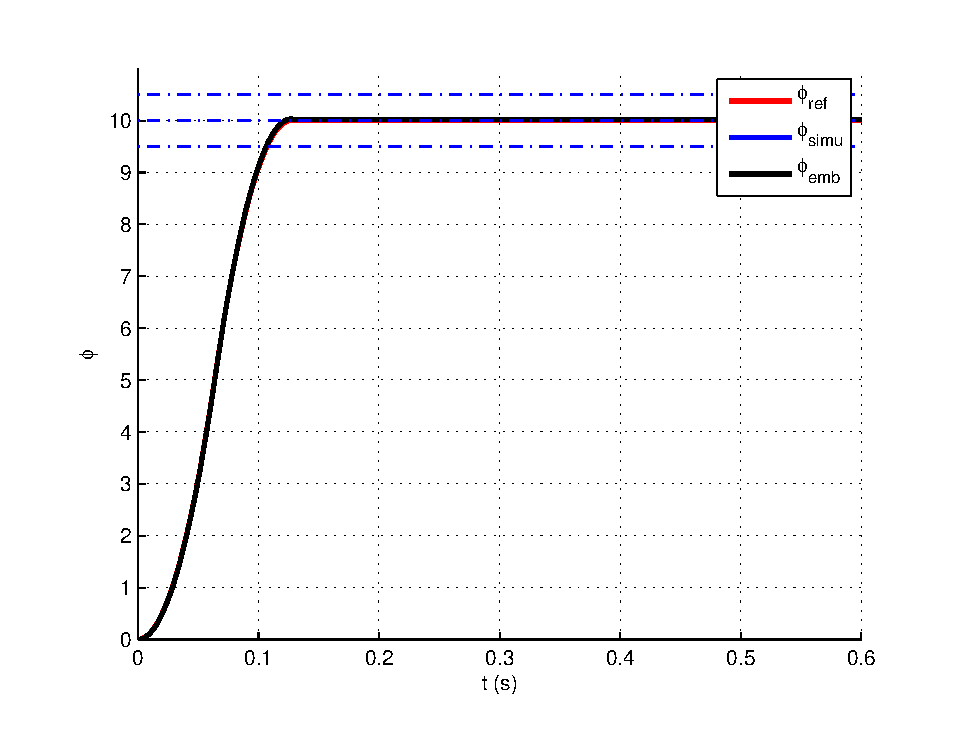
\includegraphics[width=\columnwidth]{fig/embeddedlvl110.eps}
   \caption{$Rs = 10$[rad]}
  \end{subfigure}
  \begin{subfigure}[b]{\linewidth}
  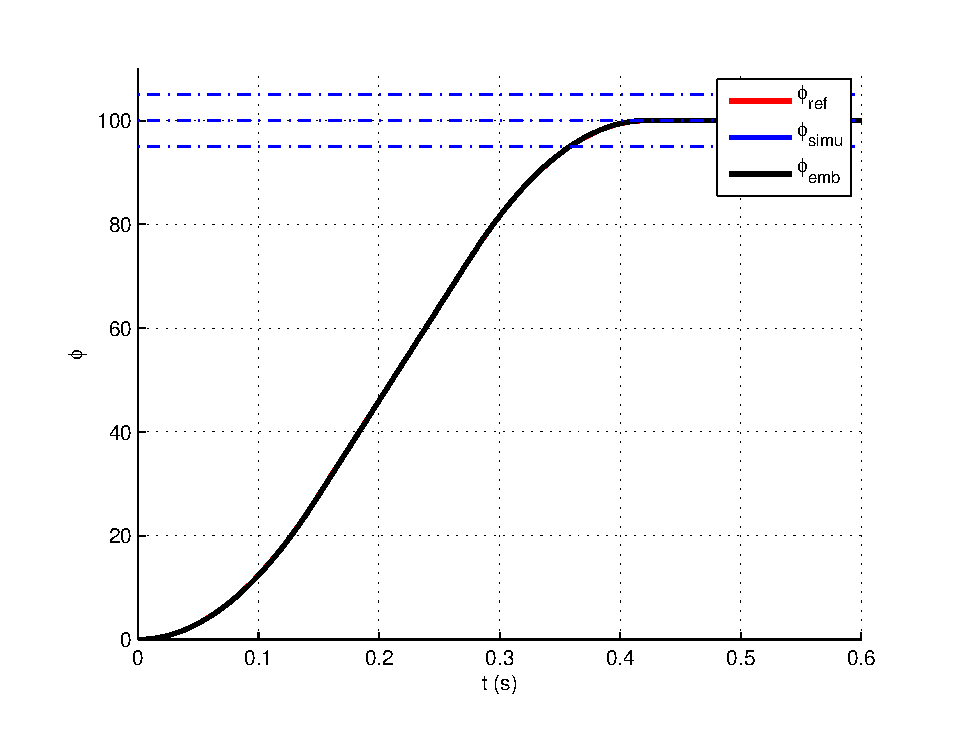
\includegraphics[width=\columnwidth]{fig/embeddedlvl1100.eps}
   \caption{$Rs = 100$[rad]}
  \end{subfigure}

 \caption{Result with a embedded controller}
 \label{embedded}
\end{figure}

%------------------------------------------------
% 		LEVEL 2
%------------------------------------------------
\subsection*{Level 2}
\addcontentsline{toc}{subsection}{Level 2}

Once we had the model following controller with both Simulink and embedded Matlab implementation, we ran it on the real motor. Figure \ref{realresults} shows the two step responses, using the two differents methods. As previously, the two curves are entirely merged.

Moreover, since our controller is designed in such a way that the motor is accelerating at $0.75 a_{max}$ and moving at most at a velocity of $0.75 v_{max}$, the trajectory planner provide safe trajectories. The step response are therefore almost the same as the one simulated.

\begin{figure}[hb]
  \centering
 \begin{subfigure}[b]{\linewidth}
 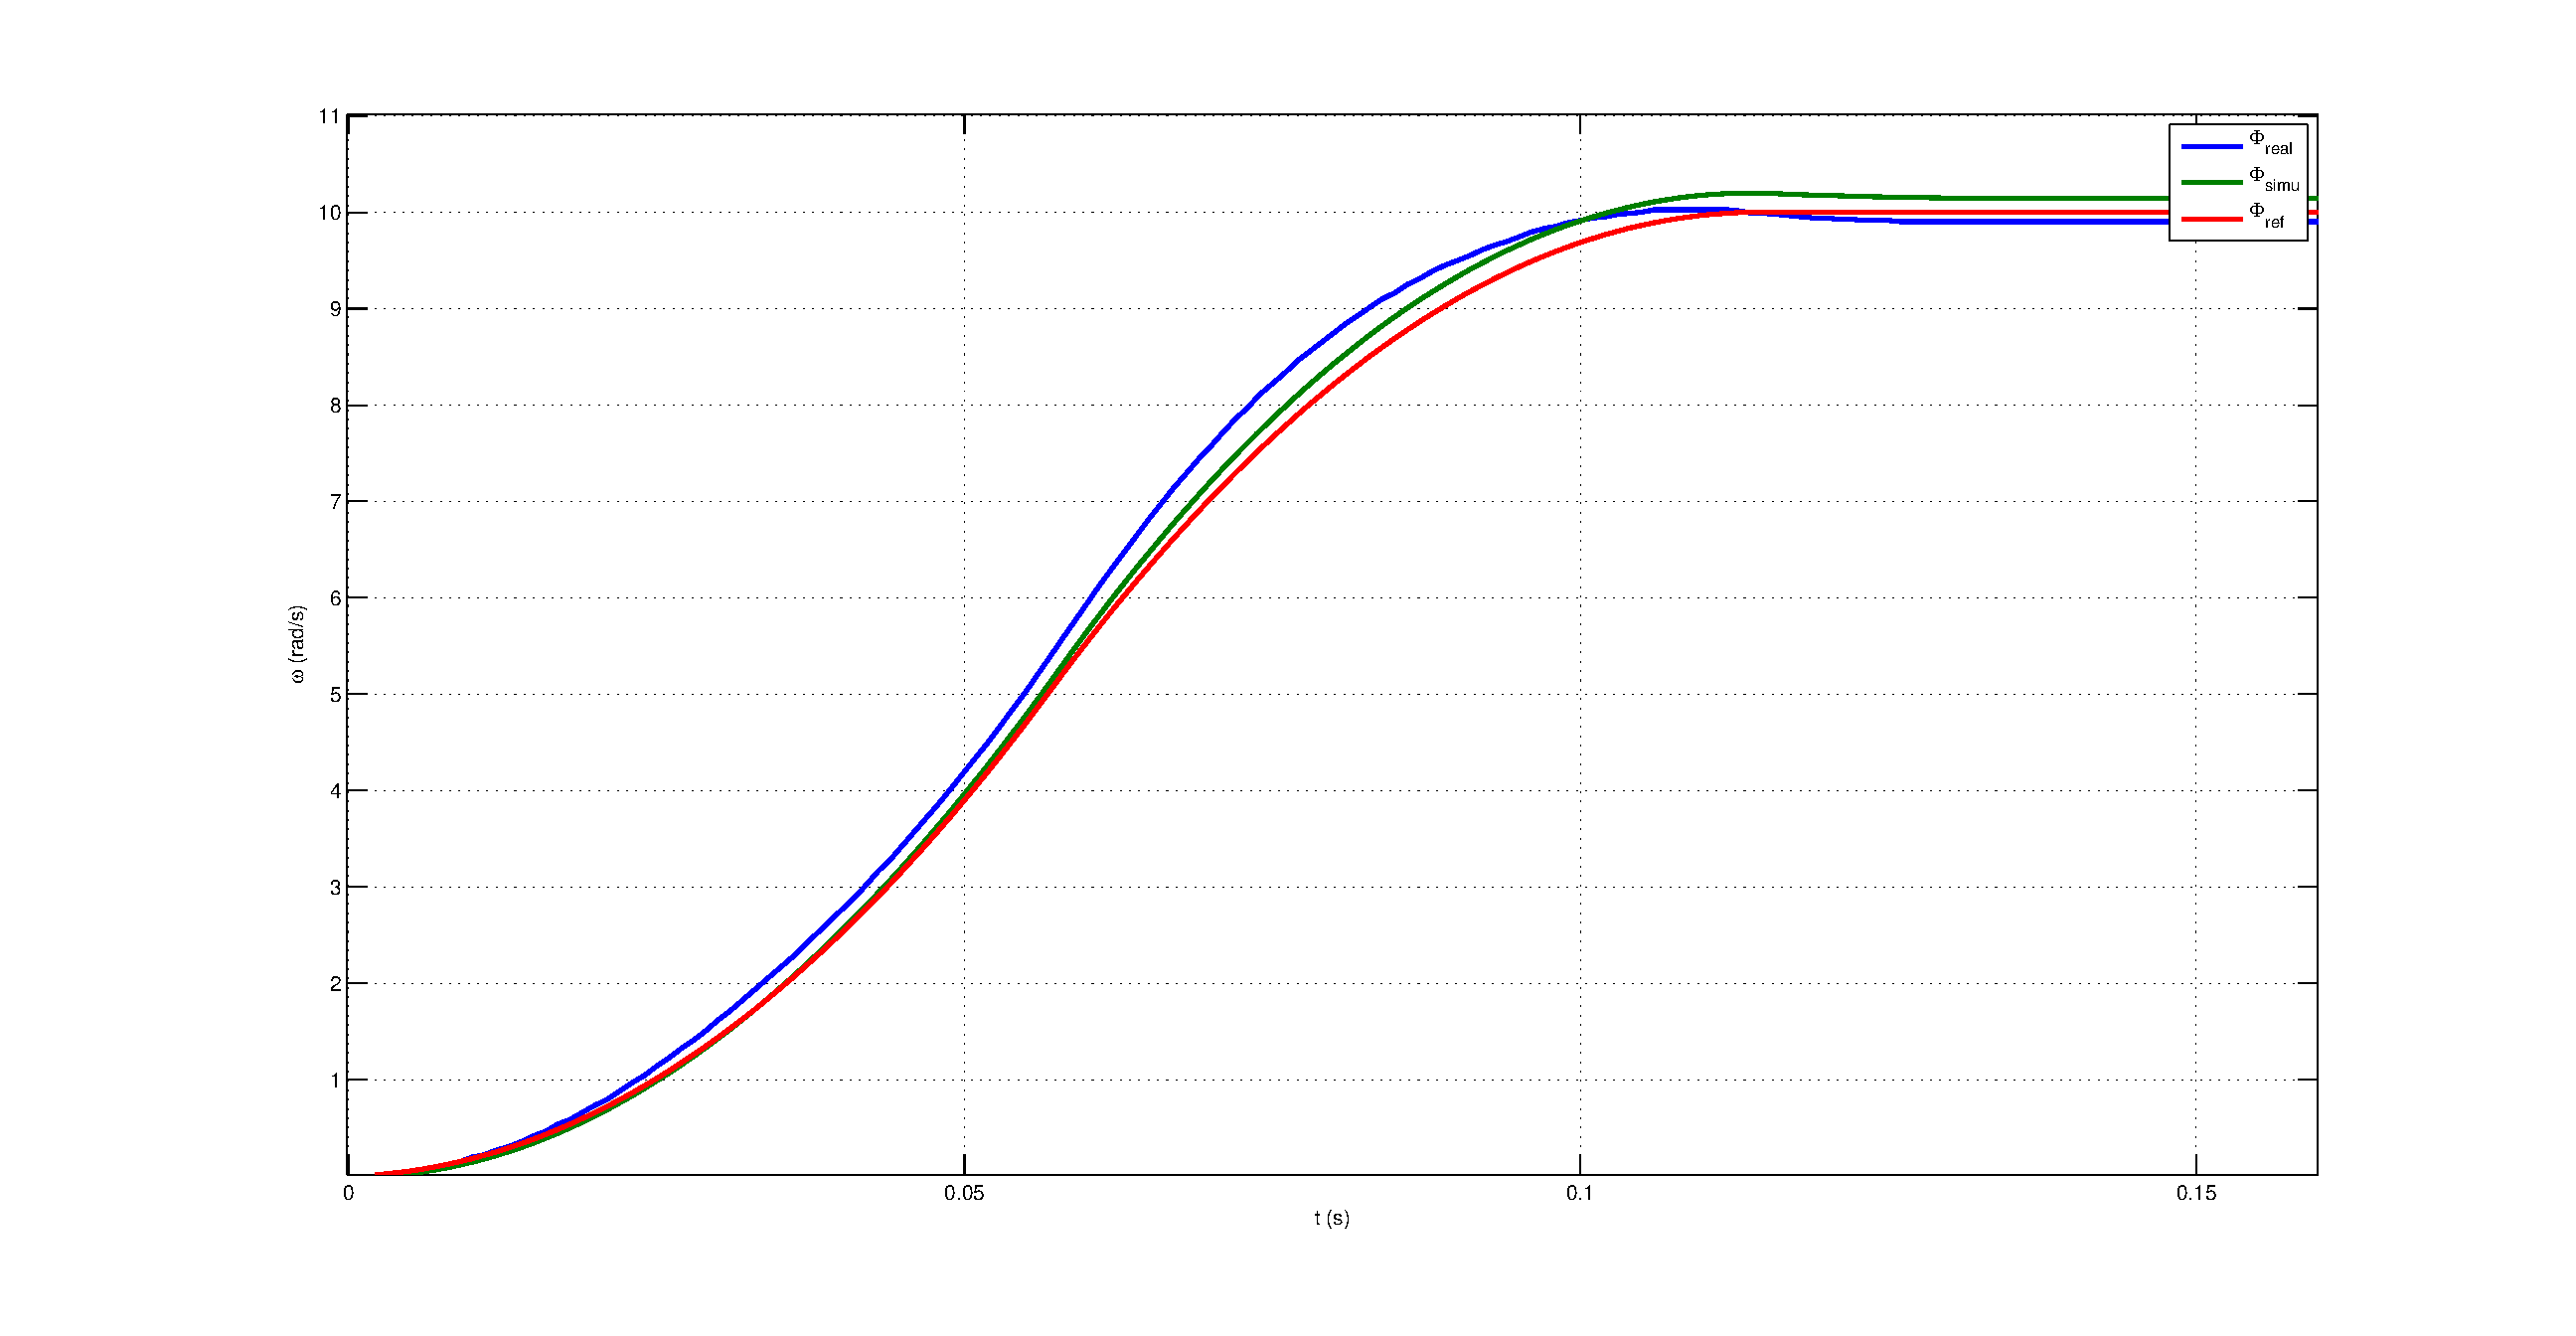
\includegraphics[width=\columnwidth]{fig/10rad.eps}
 \caption{$R_s = 10\text{[rad]}$}
 \end{subfigure}
 \begin{subfigure}[b]{\linewidth}
 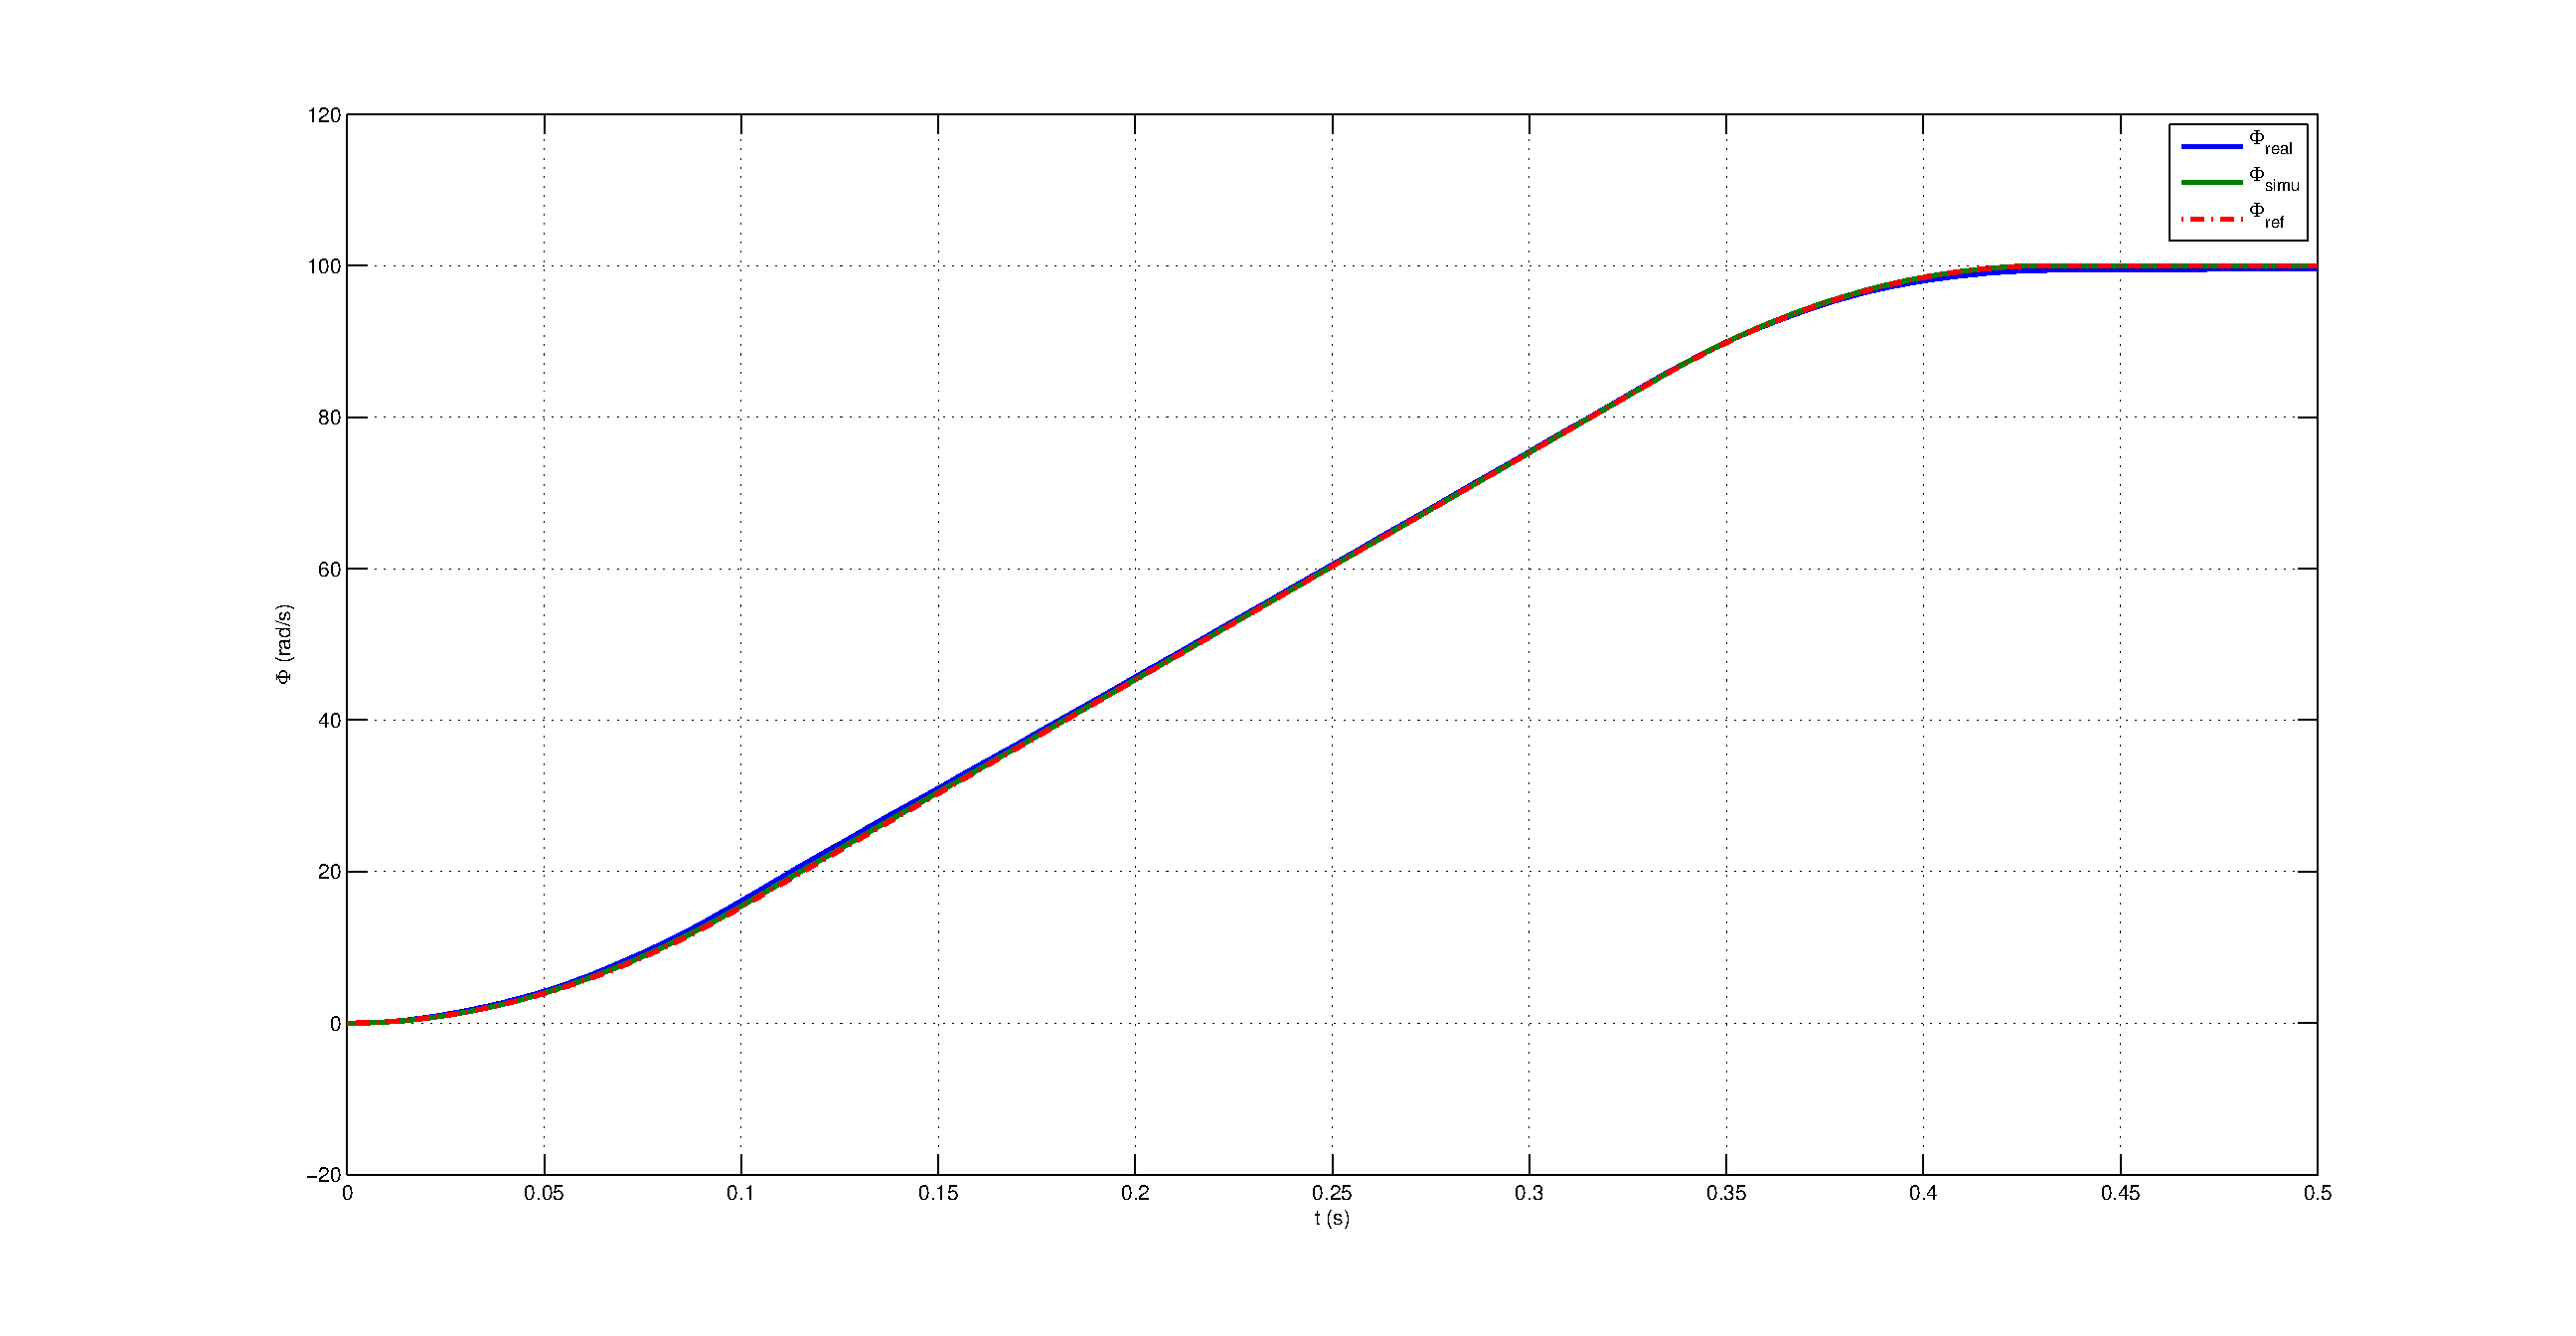
\includegraphics[width=\columnwidth]{fig/100rad.eps}
 \caption{$R_s = 100\text{[rad]}$}
 \end{subfigure}
 \caption{Simulation and real results \\ (blue) -- \\ (green) --}
 \label{realresults}
\end{figure}
	

\clearpage

\end{document}
